%%%%%%%%%%%%%%%%%%%%%%%%%%%%%%%%%%%%%%%%%%%%%%%%%%%%%%%%%%%%%%%%%%%%%%%%%%%
%
% Plantilla para un artículo en LaTeX en español.
%
%%%%%%%%%%%%%%%%%%%%%%%%%%%%%%%%%%%%%%%%%%%%%%%%%%%%%%%%%%%%%%%%%%%%%%%%%%%
\documentclass[runningheads]{llncs}
%
\usepackage{graphicx}
\usepackage{csquotes}
% Qué tipo de documento estamos por comenzar:
%\documentclass[a4paper]{article}
% Esto es para poder escribir acentos directamente:
\usepackage[utf8]{inputenc}
\usepackage[T1]{fontenc}
% Esto es para que el LaTeX sepa que el texto está en español:
\usepackage[spanish]{babel}

\def\spanishoperators{}
\selectlanguage{spanish}

%% Paquetes de la AMS
\usepackage{amsmath, amsthm, amsfonts}
%% Para añadir archivos con extensión pdf, jpg, png or tif
\graphicspath{ {images/} }
\usepackage[colorinlistoftodos]{todonotes}
\usepackage[colorlinks=true, allcolors=blue]{hyperref}

\def\keywordname{{\bf Palabras Claves:}}

\begin{document}
\pagestyle{empty}% para eliminar los encabezados y pie de paginas
%% Primero escribimos el título
\title{Empoderando Personas a Través del Uso de Internet - VIDUC}
\author{Gustavo Calcaterra, Fatima Romero
y María E. García-Díaz\\}

\authorrunning{}

\institute{Universidad Nacional de Asunción-Facultad Politécnica\\
Asunción, Paraguay\\
\email{gcalcaterra@pol.una.py, flromero@est.pol.una.py, mgarcia@pol.una.py}\\
\url{http://www.pol.una.py} }


%% Después del "preámbulo", podemos empezar el documento

%% Hay que decirle que incluya el título en el documento
\maketitle

%% Aquí podemos añadir un resumen del trabajo (o del artículo en su caso) 
\begin{abstract}

Existe un porcentaje significativo de personas con acceso a Internet o con capacidad económica de acceder a la red que no lo utiliza de una manera consciente para mejorar su calidad de vida; esto ocurre por distintas razones, entre ellas el conocimiento de uso, impacto y la aceptación cultural así como la adopción local.\cite{5}

Internet es una herramienta poderosa para aprender y desarrollar habilidades de cualquier índole como cocina, deportes, manualidades; solo por citar algunas. Mediante este trabajo se busca descubrir una forma en la que se pueda potenciar y empoderar a las personas a través del uso de Internet de manera educativa, consciente y útil.

Para poder experimentar la idea, se desarrolló una primera versión de la plataforma web, VIDUC (Vídeos Educativos, http://viduc.net), cuyo objetivo es mostrar el potencial de Internet para aprender. La plataforma filtra y ordena contenidos específicos de vídeos de Youtube, mostrando contenidos que pueden ser de interés a los usuarios. El experimento está dirigido a personas de cualquier edad que puedan acceder a Internet y que tengan pocos conocimientos sobre como utilizar la red de manera más efectiva.

A través de encuestas realizadas se encontró que a un gran porcentaje de personas le pareció de utilidad la aplicación. Potenciar el uso eficiente de Internet, buscando la educación, el empoderamiento, la autonomía, el desarrollo y la alfabetización digital de las personas es útil, ya que  ayuda a disminuir la brecha digital existente, entre otros factores positivos. La plataforma VIDUC es un caso básico que se enfoca en el contenido de vídeos para aprender nuevas habilidades así como conocer experiencias de otras personas que han podido utilizar sus habilidades para emprender negocios o resolver algunos de sus problemas.\\

%\textbf{Abstract} There is a percentage of people  with Internet access or with the economic capacity to access the Internet and these people don't use it in a conscious way to improve their lifes. This occurs for several reasons, the two that we focus here are can be put into two categories: skills, awareness and cultural acceptance; and local adoption and use.

%The Internet is a powerful tool to learn and develop skills for a variety of jobs like: cooking, sports, handcrafts, just to name some. With this research, plus understanding the actual situation in the world and in Paraguay about the Internet use, the goal is to look for ways to promote and empower people through the use of Internet in an educational, conscious and useful way.

%To develop an experiment with this idea, a first version of a Web Platform was made, VIDUC (Educational Videos, http://viduc.net), its goal is to filter and specific useful and educational content from youtube to the user. It uses the YouTube Api. The experiment is for people of any age, who have little knowledge of how to use the Web. 

%54.9\% of the surveyed people said that they would use the platform VIDUC to learn more. With this reassurance, we know is useful to enhance the healthy use and colaboration in the Internet, looking for education, empowerment, development and improving the digital literacy of people, so in this way the digital divide can be overcome. The web platform VIDUC is a basic case with a focus con video content, of course, it can have new features to provide and enhance the sharing content through  text, audio and images.


\keywords{Educación Digital \and Alfabetización Digital \and Herramienta Digital \and Brecha Digital \and Habilidades Técnicas \and Aprendizaje en Red}
\end{abstract}



%% Iniciamos "secciones" que servirán como subtítulos
%% Nota que hay otra manera de añadir acentos
\section{Introducción}

Los datos publicados por la Dirección General de Estadísticas, Encuesta y Censo (DGEEC) en setiembre del 2018 confirma que la población juvenil paraguaya de entre 15 a 29 años de edad representa el 27,79 \% de la población total, del cual 1.909.947 personas distribuidas entre hombres y mujeres tienen acceso a Internet, la encuesta demuestra que el 82,48 \% del total de personas tiene acceso a una herramienta digital, y el 17,50 \% no tiene la posibilidad de acceder a Internet.\cite{1}

Hoy en día en el Paraguay el 96,7 \% de la población total cuenta con un teléfono móvil, superando ampliando a la telefonía fija y el 24,8 \% tiene acceso a una red de Internet en su hogar, lo cual demuestra el crecimiento a nivel de acceso al mundo web de la población paraguaya. Además, se afirma que un alto porcentaje de esta población accede a las redes sociales.\cite{2} 

Así mismo, es importante mencionar que 6 de cada 10 paraguayos se dedican a actividades informales, como sub empleos, lo cual implica que muchas veces estas personas no perciban ni siquiera el salario mínimo y trabajen en condiciones no deseadas, sin tener acceso a los servicios básicos como salud y educación.\cite{12}

Este trabajo surge debido a la problemática observada de que la falta de instrumentos para identificar y segmentar aprendizajes a través de la web, con la finalidad de adquirir conocimientos y habilidades técnicas respecto a oficios en general. Según el BID, el futuro del trabajo está marcado por dos grandes tendencias, el “tsunami” tecnológico y el envejecimiento poblacional, para América Latina y el Caribe. Ambas tendencias tienen una naturaleza positiva (nos dan la posibilidad de vivir más años, abandonar los trabajos más repetitivos y aumentar nuestra calidad de vida) y presenta una gran oportunidad para la región. El futuro del trabajo no es un escenario predefinido, sino una realidad en construcción. El mercado laboral del mañana en nuestra región depende, en realidad, de cómo actuemos en todo los niveles: los estados, las empresas, los trabajadores, las escuelas, etc. \cite{3}

Se estima que la propuesta permitirá advertir no solo el potencial de las TIC en los procesos de enseñanza y aprendizaje sino también el amplio camino de ensayo y prueba que los docentes pueden recorrer en bien de las experiencias de formación profesional de los estudiantes. \cite{4}

El resto del documento está estructurado de la siguiente manera: La Sección 2 presenta información de antecedentes y trabajos relacionados en el área. La Sección 3 presenta el experimento y la solución planteada. La sección 4 presenta la validez de los datos y la interpretación de los resultados. Finalmente, en la sección 5 se presentan
las conclusiones y algunas propuestas futuras para la continuidad de esta investigación.


\section{Estado del Arte}

En esta sección se detallan los trabajos relacionados con la propuesta y que sirven de antecedentes para fundamentar la importancia de realizar este proyecto. 

\textbf{\textit{Internet for All A Framework for Accelerating Internet Access and Adoption}}\\
Este documento, que es parte del pilar Acceso/Adopción de la iniciativa Desafío Global del Foro Económico Mundial en el Futuro de Internet, provee un marco de referencia para tratar las barreras relacionadas con lograr un Internet para todos. La solución que plantea se divide en estos 4 puntos sobre como atacar la brecha digital: a) Infraestructura, b) Costo, c) Conocimiento de uso e impacto y aceptación cultural y d) Adopción local y uso. Los puntos más relevantes para esta investigación son los puntos c y d.\cite{5}

\textbf{Desafíos de la Educación Digital}\\
La nueva Ley de Protección de Datos (Ley Orgánica 3/2018, de 5 de diciembre) que rige en la Unión Europea indica que, además de adaptar la normativa interna en materia del derecho fundamental de protección de datos personales al RGPD (Reglamento General de Protección de Datos), recogió un amplio catálogo de “derechos digitales”, entre los cuales se encuentra uno de particular relevancia para hacer frente a la revolución tecnológica que está llamando a la puerta: el derecho a la educación digital, regulado en el artículo 83 del citado texto normativo. Explica el redactor, de acuerdo al artículo, el sistema educativo garantizará la plena inserción del alumnado en la sociedad digital y que el aprendizaje del uso de los medios digitales sea seguro.\cite{6}

\textbf{Los vídeos que animan al estudio en YouTube crecen un 120\% en España durante 2018}\\
Los vídeos publicados en España desde la plataforma YouTube con temática relacionada con el estudio aumentaron en un 120\% su número de visualizaciones durante el pasado año 2018 con respecto a los datos de 2017. Los vídeos de YouTube que incluyen en su título los términos 'estudia conmigo' o '\textit{study with me}', que suelen ser las búsquedas más frecuentes de los estudiantes, crecieron un 120\% entre 2017 y 2018, según datos compartidos en el estudio. Además, siete de cada diez personas que acceden a YouTube lo hacen buscando aprender algo.\cite{7} Esta publicación fundamenta con mayor fuerza la propuesta de trabajo que se presenta en este artículo.

\textbf{YouTube y su popularidad como plataforma educativa}\\
En esta plataforma se puede encontrar contenidos educativos de materias como física, matemáticas, tecnología e inglés y sus picos más altos de popularidad se dan en época de exámenes. El incremento en la popularidad de este tipo de contenidos va de la mano con la idea de la educación continua, ya que pone al alcance el conocimiento de distintas áreas, sin tener que salir de su casa.\cite{8}


\textbf{{El Futuro del Trabajo en América Latina y el Caribe. ¿Una gran oportunidad para la región?}} \\
La tecnología y la demografía son dos puntos que tienen un impacto en el presente y en el futuro en cuanto al trabajo. Los autores presentan algunos puntos sobre cómo enfrentar los desafíos, indican que se debe aplicar los cambios a nivel de estado, empresas e individuos, entre ellos mencionan que todos los individuos deben aprender todo el tiempo. Su objetivo es presentar problemáticas e ideas sobre el Trabajo en América Latina y el Caribe, para generar conciencia y acciones en los organismos más importantes. Plantea ideas sobre la automatización, la demografía y la cuarta revolución de la tecnología y cómo esto puede influir en el trabajo de mucha gente.\cite{3}

\textbf{Impacto y Aprovechamiento de las Tecnologías de la Información y las Comunicaciones en la Educación Superior} \\
En este estudio, se comprobó mediante una encuesta que el Internet es un recurso muy útil a nivel de educación, se encontró que algunos de los factores que contribuyen al uso del Internet son: el uso de la computadora del hogar, la forma divertida de usar la computadora, así como el uso de las redes sociales para chatear, también el uso de la computadora en la escuela y las redes sociales como medio de comunicación. Sin embargo, no puede desconocerse que las redes sociales y vídeos como pasatiempos en horas de ocio y horario académico actúan como distractores negativos.\cite{9}

\textbf{Construcción de un instrumento para el aprendizaje en red de estudiantes universitarios}\\
Este artículo justifica la investigación basándose en la falta de instrumentos para identificar aprendizajes en la red y desarrollar habilidades de búsqueda de información al interactuar en ese medio, se procura orientar las prácticas de enseñanza de los docentes. En tal sentido, se presentan los datos de una prueba piloto que se realizó para identificar cómo los estudiantes de la Universidad Autónoma de Sinaloa se apropian de los aprendizajes cuando interactúan en Internet y cuáles habilidades desarrollan cuando buscan información en ese medio digital. Los resultados demuestran que aproximadamente 50 \% de los jóvenes conectados a la Red autorregula su aprendizaje, más de 90 \% se siente motivado cuando busca información en la Web y más de la mitad comprende cómo las TIC fomentan el aprendizaje.\cite{10}

\textbf{Invertirá YouTube 20 millones de dólares en recursos para EduTubers?} \\
YouTube financiará a EduTubers para crear contenido en temas referentes a habilidades profesionales, como tutoriales para el desarrollo de currículums, cursos de programación de videojuegos o clases de JavaScript. Es indudable que YouTube es un poderoso espacio de aprendizaje para todo tipo de público; en esta plataforma se puede aprender desde cómo reparar una lavadora o cómo cocinar arroz, hasta diseñar modelos en 3D o páginas web. Sin embargo, la mayoría de su contenido está bajo constante crítica por la falta de calidad y control.\cite{11} 

\textbf{Encuesta sobre acceso y uso de Internet en Paraguay}\\
Esta encuesta se realizo por la Secretaría Nacional de Tecnologías de la Información y Comunicación (SENATICs) en el año 2017 en Paraguay, con una muestra representativa de personas de la Capital y de 14 Departamentos por la empresa First Análisis y Estudios. Los resultados tienen un margen de error de +-3,5\% y un índice de confianza del 95\%. Entre otros puntos confirma que de las personas distribuidas entre hombres y mujeres del Paraguay, un 86,9 \% tiene acceso a Internet a través de una computadora o un celular.\cite{2} 

\textbf{Informalidad laboral desafiante en Paraguay}\\
La situación de la República del Paraguay en cuanto a los indicadores de la población que realizan trabajos informales tomando como referencia el año 2010 al 2016. La informalidad laboral no es "propiedad exclusiva de Paraguay", sino un flagelo que se observa en todo el mundo. Sin embargo, en el país se registran cifras alarmantes, especialmente en las pequeñas y medianas empresas, y en áreas como la construcción, el comercio, el servicio doméstico, entre otros.\cite{12}\\
Por ello es importante resaltar que la plataforma VIDUC puede aportar formación empírica a los usuarios en cuanto a los diversos oficios o intereses y a su vez ser una fuente importante de conocimiento que permita el desarrollo personal apuntando a mejores trabajos, entre ellos formales.

\section{Propuesta de Solución}
Se implementa un diseño descriptivo al ser una investigación social. Se ha optado por el desarrollo de una plataforma web para ejecutar el experimento aplicando la combinación de técnicas cuantitativas y cualitativas a través de una encuesta que permita reunir una serie de datos útiles que apoyarán el estudio. 
A continuación se explica en detalle el proceso llevado a cabo, tanto para la elección de la población a ser encuestada, seguidamente los instrumentos utilizados para fundamentar los resultados y el procedimiento aplicado, así como también la plataforma tecnológica utilizada en el desarrollo de la aplicación.

\subsection{Arquitectura Tecnológica}
La plataforma se elaboró con el Framework CAKE PHP \cite{15}. Se utilizó como contribución al diseño web: Html5, JQuery y CSS. Se desplegó la aplicación en un contenedor Docker \cite{17} sobre \textit{OpenShift} \cite{18} en la Nube. La aplicación se despliega sobre un Apache\cite{19} y utiliza una base de datos MySQL\cite{20}. El diseño utilizado es Modelo - Vista - Controlador (MVC), es orientado a objetos y es una aplicación web. El código fuente se encuentra en GitHub.\cite{22}\\
\textbf{Funcionalidades: }La funcionalidad principal es llamar a la API de Youtube\cite{21} para mostrarle al usuario videos filtrados de educación que le pueden ser de interés.\\
\textbf{Calidad de Código: }Se utilizo la plataforma de software libre SONARQUBE \cite{13} para evaluar la calidad del código fuente del Proyecto VIDUC, realizando un análisis estático sobre dicho código, con el objetivo de advertir sobre diferentes puntos a mejorar. En el resultado salió un Ratio de «Deuda Técnica» menor al 10\%, por tal motivo se considera que el proyecto VIDUC está sano.

\subsection{Población de la Muestra}
La muestra está compuesta de 51 personas sin grado de formación universitaria de ambos géneros, la mayor cantidad 61\% femenino y 39 \% masculino, cuyas edades comprenden entre los 15 y 44 años. En cuanto a nivel de formación académica el 78\% es nivel secundario y el 21\% con educación secundaria inconclusa.
\begin{figure}[h]
\caption{Gráfico \% Formación Académica de la Muestra}
\centering
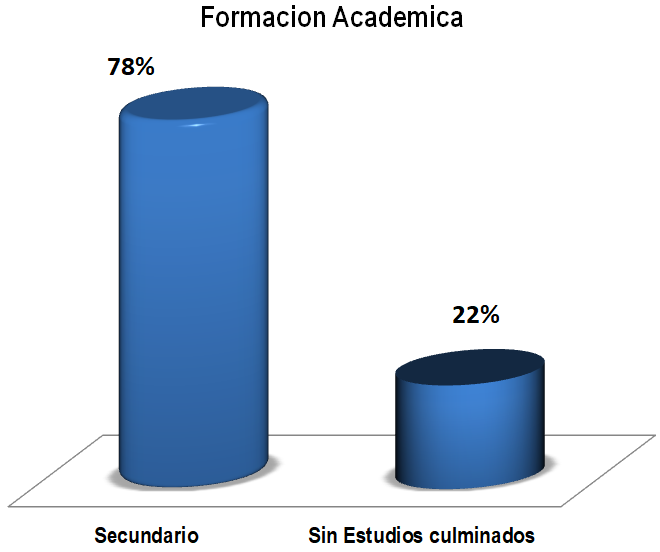
\includegraphics[width=7cm, height=5cm]{muestragenero.PNG}
\end{figure}

\subsection{Instrumentos}
Se elabora un prototipo de aplicación \textit{online} denominado VIDUC (Vídeos Educativos) con el fin de que sea usado como herramienta para adquirir nuevos conocimientos y conocer el potencial de utilizar vídeos para aprender. Se puede acceder a través de la url: http://viduc.net.
Complementando el trabajo realizado se seleccionó la metodología de encuestas que fue direccionado principalmente a los alumnos del programa Tenondera, se explica sobre el programa más adelante.
En el cuestionario se analiza una serie de áreas consideradas de relevancia para la investigación\href{https://forms.gle/JvFyK6oAv7Ca7vGF9/}{(Ver Encuesta)}. La encuesta fue elegida para recopilar información sobre aspectos difíciles de observar directamente por el investigador. Es un instrumento muy adecuado para desarrollar el conocimiento de la conducta y los procesos educativos, así como para el estudio aplicado a las características de una población reducida.
\subsection{Proceso experimental}
El procedimiento en general del trabajo para completar el experimento es:
\begin{enumerate}
    \item Probar y verificar las funcionalidades de la plataforma VIDUC antes de su puesta en producción, que la misma cumpla con los requerimientos pre-establecidos en su configuración.
    \item Redactar la encuesta con el objetivo recolectar datos que permitan saber puntos de interés para la investigación. Verificación y corrección de la encuesta en base a los requerimientos finales de la plataforma.
    \item Seleccionar la muestra, que fue los alumnos del programa Tenonderá, atendiendo que los mismos son de escasos recursos y a través de la utilización de la plataforma VIDUC podrían adquirir conocimientos sobre temas de interés que les ayuden en su crecimiento personal y progreso económico.
    \item Preparar el instructivo a seguir para realizar el experimento a fin de evitar la pérdida de información relevante para la investigación.
    \item Realizar el experimento en una ambiente controlado (sala de informática de la Facultad Politécnica de la UNA) siguiendo la secuencia de tiempo establecido por los coordinadores del programa Tenonderá.
    \item Verificar los datos recolectados, si se completo todos los campos pre-establecidos correctamente.
    \item Analizar los resultados obtenidos de acuerdo a los parámetros establecidos en las plataforma VIDUC.
\end{enumerate}
%\subsection{Experimento}
La recolección de datos se llevó  a cabo a través del llenado del Formulario \textit{Online Google Forms}, la encuesta se realizó en las instalaciones de la Facultad Politécnica de la Universidad Nacional de Asunción  en el marco del Programa denominado TENONDERÁ, que tiene el fin de propiciar el crecimiento académico de los jóvenes de los últimos años de los cursos de la media, en instituciones que no cuentan con suficiente recursos de acceso a tecnología, proporcionándoles opciones de capacitación en las herramientas ofimáticas, demandadas en el mercado laboral\cite{15}.
Luego se procedió a la aplicación del experimento el cual tuvo una duración de 30 minutos. Se implementó la prueba, que incluyó algunas indicaciones, preguntas y respuestas y se mostró donde acceder a la encuesta.
También se le compartió la aplicación y la encuesta a otras personas externas al grupo Tenonderá para tener más diversidad de personas y de edad. Se aclara que la aplicación y la encuesta está disponible en Internet. Para el análisis de datos se definió un cierre para no mezclar con nuevos datos.

\section{Resultados}
El trabajo se desarrolla en base a la utilización de la aplicación VIDUC (Vídeos Educativos) y mediante el llenado del Formulario \textit{Online Google From} en donde se toma como referencia preguntas direccionadas sobre la utilización de Internet, y la posibilidad de aprender diversos conocimientos, el cual arroja como resultado que actualmente en Paraguay hay un porcentaje elevado de personas que tienen acceso a Internet, a través de diversos dispositivos, como es el caso de las personas encuestadas mediante la investigación. De un total de 51 encuestados un 63\% representa mujeres y un 37\% varones.

A través de este trabajo se verifica que un importante número de personas le pareció de utilidad la aplicación. Por ende se resalta el hecho de que es útil potenciar un uso saludable de Internet, buscando la educación, el empoderamiento, el desarrollo y la alfabetización digital de las personas para disminuir en algo la brecha digital existente. La plataforma VIDUC es un caso básico que se enfoca en el contenido de vídeos, se podría aplicar mejoras para potenciar otras maneras de compartir contenido como por ejemplo: texto, audio, imágenes, entre otros.
\begin{figure}[h]
\caption{Gráfico sobre el \% referente a la encuesta realizada}
\centering
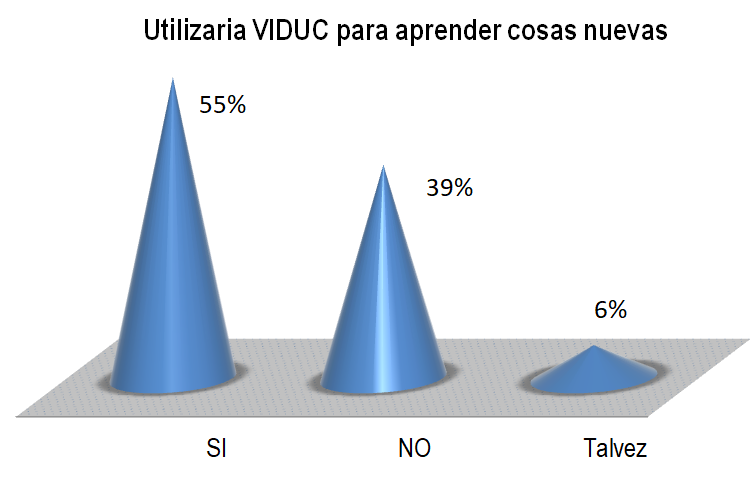
\includegraphics[width=9cm, height=5cm]{viduc.PNG}
\end{figure}

Según la muestra indica que un 94\% de los encuestados tienen acceso a internet lo cual indica un crecimiento importante a nivel país en cuanto a la utilización de herramientas digitales. Se comprobó que un 93.1 \% de los encuestados utilizan internet desde su teléfono móvil, y un 78.4\% afirmó  que lo utiliza diariamente.

También se pudo comprobar que el uso de Internet se enfoca en la distracción ya que el 78.4 \% utiliza en redes sociales y  distracciones varias, y sólo el 22.1 \% se enfoca en educación y adquirir nuevos conocimientos. Un razón desfavorable para el uso de Internet podría ser el hecho de que el 78.9\% de los encuestados indicaron que no confían en la información encuentran en Internet.

No se puede dejar de mencionar que gran parte de las personas encuestadas tienen la opinión que pueden aprender cosas nuevas; de éstos el 84.3\% opinan que sí puede aprender en Internet. Se confirma que el 57.7 \% afirma que no está seguro que le den un buen uso al Internet, pero mencionan que forma parte de un hábito diario.

En la figura 2 se observa que el 55\% utilizaría VIDUC como herramienta para aprender nuevas habilidades. El 79.6\% de los encuestados sienten que pueden aprender a través de videos y el 72.2\% opta por recibir contenidos a través de vídeos, capaz por la facilidad de captar la atención y sencillez para comprender los contenidos.

Se confirma de esta manera  que el uso de internet es algo que ya es un hábito que se practica  en la sociedad del presente para cuestiones relacionadas con la vida diaria e incluso para aprender nuevas capacidades y adquirir nuevas competencias.

\section{Conclusiones y Trabajos Futuros}
Del análisis realizado, se afirma que el acceso a Internet forma parte de un hábito diario. La cuestión preocupante es que una gran mayoría no enfoca al máximo el aprovechamiento del Internet por distintas razones, desconocimiento de uso, fuente no confiable, desconocimiento de que existe en la web, entre otros. Y por ende no saben filtrar, diferenciar e interactuar con los contenidos que se encuentran disponibles en Internet. Se confirma que hace falta un mejor aprovechamiento de esta herramienta que es Internet, mover a las personas de su zona de confort, inculcar y motivarlas a la utilización más consciente de Internet para que puedan desarrollarse en sus propios temas de interés, problemas y dudas.

VIDUC, como parte de la investigación, es una herramienta que busca empoderar y motivar a las personas a aprender algún oficio, habilidad o técnica a través del uso de Internet. Su objetivo es filtrar contenidos de vídeo sin distracciones para motivar y mostrar que se puede aprender y encontrar contenidos útiles en internet. Las personas encuestadas se sorprendieron de los temas encontrados en la plataforma. Muchos expresaron que tienen intereses pero no saben como canalizar o filtrar estos temas en la Web. Cabe resaltar que la información ya se encontraba en Internet la herramienta solo las filtró y clasificó de Youtube para así captar la atención de los usuarios y mostrarles lo que pueden aprender y poner en práctica.

%\section{Trabajos Futuros}
La proyección de la plataforma VIDUC tendría dos partes y funcionaria como un asistente. La primera le servirá al usuario para encontrar historias inspiradoras con las que se pueda identificar para avanzar e inclusive entre ellas encontrar algún mentor con el que se pueda comunicar. La segunda parte le mostrará cómo utilizar herramientas de Internet para avanzar hacia sus objetivos. A continuación, un ejemplo. El asistente le hace ciertas preguntas al usuario y aprende que esta persona tiene pocos recursos económicos y que le gustaría ser Chef. Entonces la plataforma le presentará la historia de una persona que pudo avanzar en la cocina con circunstancias parecidas al de esta persona para que se sienta inspirada y observe lo factible que son sus aspiraciones. Luego la plataforma le mostrará una serie de maneras de utilizar Internet para aprender habilidades de cocina, como canales de YouTube de cocina, blogs de Chefs, etc. La plataforma también podría tener la capacidad de que los mentores o personas que cuentan su historia, así como las personas que buscan aprender, puedan conectarse entre sí o por lo menos tener los enlaces para poder conectarse en otras plataformas externas.\\
%La plataforma podría ir aprendiendo de acuerdo a las búsquedas y cómo va utilizando la plataforma para sugerirle nuevas maneras de cómo puede utilizar Internet para su propio beneficio. Lo más básico de este punto sería, a través del feedback y el historial del usuario, le recomendará vídeos relacionados.


 %\newpage
\begin{thebibliography}{20}

\bibitem{1}
Secretaría Nacional de Tecnologías de la Información y Comunicación:DGEEC comparte datos sobre la población juvenil en Paraguay, \url{https://www.dgeec.gov.py/news/DGEEC-comparte-datos-sobre-la-poblacion-juvenil-en-Paraguay.php},(2018) Accedido 14 Febrero 2019

\bibitem{2}
Secretaría Nacional de Tecnologías de la Información y Comunicación:Encuesta sobre acceso y uso de Internet en Paraguay, \url{http://gestordocumental.senatics.gov.py/share/s/ntjnuNLeT8u3gbAHC6WeVw},(2017) Accedido 20 May 2019

\bibitem{3}
Bosch M.,Pagés ,C., Ripani, L.: El futuro del trabajo en América Latina y el Caribe. Banco Interamericano de Desarrollo,pp. 04-10
 \url{http://dx.doi.org/10.18235/0001340}(2018).
 
\bibitem{4}
Tumino, M.,Bournissen ,J., Forneron, F.: Validación de contenido de instrumentos para medir el
nivel de integración tecnológica en el aula y el nivel de impacto en los estudiantes. Libro de     Actas CACIC2018,pp. 146-154
 \url{http://cacic2018.exa.unicen.edu.ar/}(2018).

\bibitem{5}
World Economic Forum: Internet for All - A Framework for Accelerating Internet Access and Adoption. \url{http://www3.weforum.org/docs/WEF_Internet_for_All_Framework_Accelerating_Internet_Access_Adoption_report_2016.pdf}. (2016)

\bibitem{6}
Jiménez, R.:Desafíos  de  la  educación  digital.Expansion , \url{https://hayderecho.expansion.com/2019/01/18/desafios-educacion-digital/}.(2019) Accedido 31 Jan 2019

\bibitem{7}
Europa Press:Los vídeos que animan al estudio en YouTube crecen un 120\% en España durante 2018  \url{https://www.europapress.es/portaltic/internet/noticia-videos-animan-estudio-youtube-crecen-120-espana-2018-20190208142641.html}.(2019) Accedido 30 April 2019

\bibitem{8}
Delgado, P.:YouTube y su popularidad como plataforma educativa.Tecnológico de Monterrey \url{https://observatorio.tec.mx/edu-news/youtube-y-su-popularidad-como-plataforma-educativa}.(2019) Accedido 10 May 2019

\bibitem{9}
Alcibar,M.,Monroy,A.,Jiménez,M.:Tecnologías digitales y educación para el desarrollo sostenible. Un análisis de la Producción Científica. Pixel-Bit: Revista de Medios y Educación \textbf{1}(54),  pp. 83-103(2019)

\bibitem{10}
Soto, M.: Construcción de un instrumento para el aprendizaje en red de estudiantes universitarios. Revista Iberoamericana para la Investigación y el Desarrollo Educativo, 8(16)(2019)
\doi{https://doi.org/10.23913/ride.v8i16.362}

\bibitem{11}
Guijosa, C.:Invertirá YouTube 20 millones de dólaresen recursos para EduTubers.Tecnológico de Monterrey \url{https://observatorio.tec.mx/edu-news/invertira-youtube-20-millones-de-dolares-en-edutubers}.(2018) Accedido 29 May 2019

\bibitem{12}
ABC Color: Informalidad laboral desafiante en el Paraguay, \url{http://www.abc.com.py/especiales/fin-de-semana/informalidad-laboral-desafiante-1643114.html}.(2017) Accedido 02 Jun 2019

\bibitem{13}
SonarSource S.A: Code Quality and Security, \url{https://www.sonarqube.org/}.(2019) Accedido 15 Jun 2019

\bibitem{14}
USERFOCUS: 247 web usability guidelines, \url{https://www.userfocus.co.uk/resources/guidelines.html}.(2014) Accedido 20 Jun 2019

\bibitem{15}
Facultad Politecnica UNA:ProyectoTenonderaIII, \url{https://www.pol.una.py/sites/default/files/files/extension/ProyectoTenonderaIII.pdf}.(2009) Accedido 02 July 2019

\bibitem{16}
Cake Software Foundation, Inc., \url{https://cakephp.org/}. (2019) Accedido 20 Mayo 2019.

\bibitem{17}
Docker Inc., \url{https://www.docker.com/}. (2019) Accedido 25 Mayo 2019.

\bibitem{18}
RedHat OpenShift, \url{https://www.openshift.com/}. (2019) Accedido 20 Mayo 2019.

\bibitem{19}
The Apache Software Foundation, \url{https://www.apache.org/}. (2019). Accedido 20 Mayo 2019.

\bibitem{20}
Oracle Corporation, \url{https://www.mysql.com/}. (2019). Accedido 20 Mayo 2019.

\bibitem{21}
Youtube, \url{https://www.youtube.com/}. (2019). Accedido 20 Mayo 2019.

\bibitem{22}
Código fuente de viduc-cakephp, \url{https://github.com/gcalcaterra/viduc-cakephp/}. (2019). Accedido 17 Julio 2019.

%\\bibitem{ref_lncs1}
%\Author, F., Author, S.: Title of a proceedings paper. In: Editor,
%\F., Editor, S. (eds.) CONFERENCE 2016, LNCS, vol. 9999, pp. 1--13.
%\Springer, Heidelberg (2016). \doi{10.10007/1234567890}
%\\bibitem{ref_book1}
%\Author, F., Author, S., Author, T.: Book title. 2nd edn. Publisher,
%\Location (1999)

%\\bibitem{ref_proc1}
%\Author, A.-B.: Contribution title. In: 9th International Proceedings
%\on Proceedings, pp. 1--2. Publisher, Location (2010)

%\\bibitem{ref_url1}
%\LNCS Homepage, \url{http://www.springer.com/lncs}. Last accessed 4
%\Oct 2017
%\end{thebibliography}
%\begin{thebibliography}{0}

\end{thebibliography}{}



\end{document}